%
% Module TODO:MODNUM Chapter TODO:CHAPNUM Program Documentation
% CSC160-C00: Computer Science I (C++) (Jeffrey Hemmes)
% Author: Ashton Hellwig
% Date: TODO:DATE
%


\documentclass[a4paper,11pt]{article}


  % Packages
  \usepackage[english]{babel}       % Internationalization
  \usepackage{soul}                 % Highlighting
  \usepackage{hyperref}             % Links (internal and external)
  \usepackage{fancyhdr}             % Headers and footers
  \usepackage[dvipsnames]{xcolor}   % Text Colors
  \usepackage{listings}             % Code Snippets
  \usepackage[section]{algorithm}   % List of algorithms
  \usepackage{algorithmicx}         % Algorithmic notation support
	\usepackage{algpseudocode}        % Algorithmic notation environments
	\usepackage{enumitem}             % Ordered lists
  \usepackage{geometry}             % Page layout
  \usepackage{graphicx}             % Image support
  \usepackage[toc, page]{appendix}  % Appendix
  \usepackage{amsmath}              % Mathematical Typesetting
  \usepackage{mdframed}             % Colored Boxes


  % Colors
  \newcommand{\commentstylecolor}{\color{Gray}}
  \newcommand{\keywordstylecolor}{\color{MidnightBlue}}
  \newcommand{\stringstylecolor}{\color{ForestGreen}}
  \newcommand{\questioninput}{\color{Red}}
  \newcommand{\answertcolor}{\color{Green}}
  \newcommand{\myanswer}{\answertcolor{\hl}}


  % Image Directory
  \graphicspath{ {screenshots/} }


  % Hyperlink Setup
  \hypersetup{
    colorlinks = true,
    urlcolor = blue,
    linkcolor = blue
  }


  % Syntax-Highlighting for Code Snippets
  \lstset{
    backgroundcolor=\color{white},
    breaklines=true,%
    captionpos=b,%
    frame=tb,%
    tabsize=4,%
    numbers=left,%
    showstringspaces=false,%
    commentstyle=\commentstylecolor,%
    keywordstyle=\keywordstylecolor,%
    stringstyle=\stringstylecolor%
  }


  % Page Configuration
  %% Style
  \pagestyle{fancy}

  %% Layout
  \geometry{%
  a4paper,%
  top=2.5cm,%
  bottom=2.5cm,%
  left=2.5cm,%
  right=2.5cm%
  }
  \setlength{\headheight}{15pt}
  \setlength{\floatsep}{12pt}
  \setlength{\parindent}{2em}
  \setlength{\parskip}{0.5em}
  \renewcommand{\baselinestretch}{0.75}

  %% Title page
  \title{Chapter 2 Program 1 Documentation}
  \author{Ashton Hellwig}
  \date\today
  \setcounter{tocdepth}{3}

  %% Subsequent pages
  \lhead{CSC160}
  \rhead{Computer Science I (C++)}
  \lfoot{MTODO:MODNUMCTODO:CHAPNUMProgram}
  \rfoot{A. Hellwig}


  % Document Content
\begin{document}
  % Title Page
  \maketitle
  \tableofcontents
  \listofalgorithms
  \lstlistoflistings
  \newpage


  % Problem Analysis
  \section{Problem Analysis}
    The problem states:
    \begin{mdframed}[backgroundcolor=green!20]
      This assignment relates to content from Chapter 2 of the eText.

      \textbf{Instructions}\vspace{-8pt}
      \begin{enumerate}
        \item Step One
      \end{enumerate}
    \end{mdframed}

    \subsection{Data}
      Available data includes:
      \begin{enumerate}
        \item \texttt{KnownData1}: Todo
      \end{enumerate}

    \subsection{Desired Output}
      \begin{figure}[h]
        \caption{main.cpp output}
        \begin{lstlisting}[language=bash]
Output Here
        \end{lstlisting}
        \label{fig:do}
      \end{figure}


  % Algorithm
  \newpage
  \section{Algorithm}
    Below is the algorithm for the program.
    \begin{algorithm}[h]
      \caption{Chapter TODO:CHAPNUM Program Algorithm}
      \vspace{12pt}
      \begin{algorithmic}[1]
        \Function{main}{}
          %% Variables
        \Comment{--Variables--}
          \State $num1\gets 0$
        \EndFunction
      \end{algorithmic}
      \label{alg:cTODO:CHAPNUMprogram}
    \end{algorithm}


  % User Documentation
  % \newpage
  \section{User Documentation}

    %% Usage
    \subsection{Build}
      The following are instructions with two use cases:
      \begin{itemize}
        \item With CMake
        \item Bundled Release
      \end{itemize}
      \subsubsection{With CMake}
        \begin{enumerate}
          \item Navigate to the unzipped folder containing the binary,
            \textbf{with a terminal emulator or command prompt}, this will
            (most likely) mean running:
            \begin{lstlisting}[language=bash]
cd ~/Downloads/ashellwig_csc160_programming-assignment_mTODO:MODNUMcTODO:CHAPNUM
            \end{lstlisting}
          \item Compile the program using CMake after switching to the build
            directory:
            \begin{lstlisting}[language=bash]
cd build
cmake ..
cmake --build .
            \end{lstlisting}
          \end{enumerate}
      \subsubsection{Bundled Release}
        \begin{enumerate}
          \item Navigate to the unzipped folder containing the binary,
            \textbf{with a terminal emulator or command prompt}, this will
            (most likely) mean running:
            \begin{lstlisting}[language=bash]
cd ~/Downloads/ashellwig_csc160_programming-assignment_mTODO:MODNUMcTODO:CHAPNUM
            \end{lstlisting}
          \item To run the program simply issue this within the command
            prompt
            \begin{lstlisting}[language=bash]
./build/ChapterTODO:CHAPNUMProgram
            \end{lstlisting}
        \end{enumerate}
        Of course if preferred, you may also navigate to the build folder in
          file explorer and double click the executable
          (\texttt{ChapterTODO:CHAPNUMProgram}).


  % Appendix
  % \newpage
  % \appendix

  % Images
  % \section{Images}
  %   \begin{figure}[H]
  %     \caption{Compilation and Running Program Output}
  %     \centering
  %     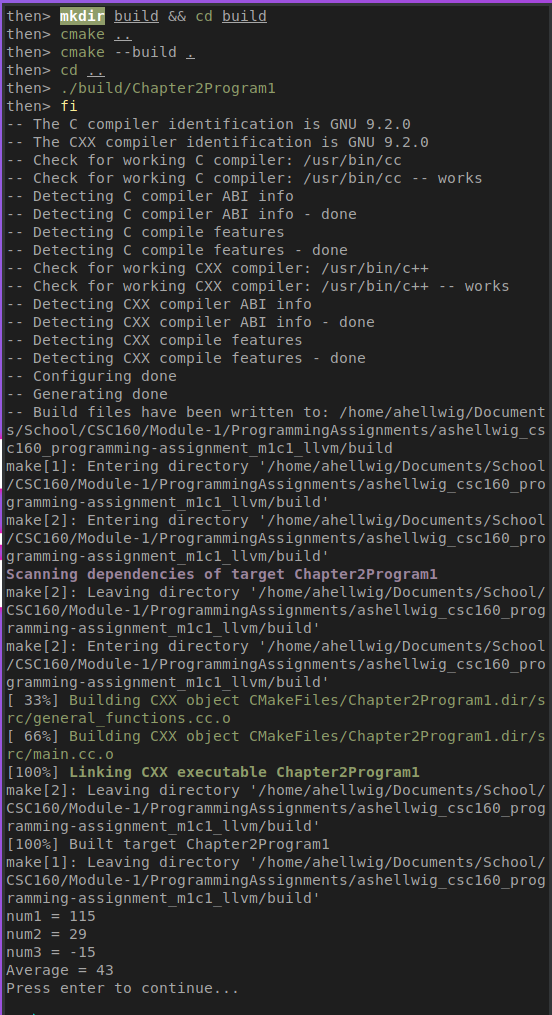
\includegraphics[%
  %       width=\textwidth,%
  %       height=600px%
  %     ]{compandrun.png}
  %   \end{figure}
\end{document}
